\subsubsection{What does it mean to be secure?}
Modern cryptography is focused on three key aspects:
\begin{enumerate}
\item \textbf{Definitions:} Concrete mathematical definition of what it means for a particular cryptographic mechanism to be secure.
\item \textbf{Schemes:} Design the schemes which will (hopefully) meet the security definitions.
\item \textbf{Proofs:} Check whether the design meets the security definitions (provable/reductionist security).
\end{enumerate}

For instance with factorization, given a large number, it is very difficult to factorize. An algorithm to do this efficiently in polynomial time would break all schemes that rely on factorization. 

\subsection{Security Games}
\textbf{Security games} are mathematical frameworks used in cryptography to formally evaluate the security of a computational problem or cryptographic system. They involve an interaction between two entities:

\begin{itemize}
    \item \textbf{The challenger}, who provides an input (e.g., a computational problem).
    \item \textbf{The adversary} (A), who attempts to solve the problem or break the cryptographic system under specific rules and constraints.
\end{itemize}

The goal is to quantify the probability of the adversary's success within a defined resource limit (like time or computational power).

\subsubsection{The FACTOR Problem}
In this example, the security game focuses on the \textbf{Factorization Problem}, where the adversary tries to factorize a large number \(N\), generated as the product of two large primes \(p\) and \(q\). \\

\textbf{Steps in the Security Game:}

\begin{enumerate}
    \item Setup by the Challenger:
    \begin{itemize}
        \item Two large primes \(p\) and \(q\) are randomly chosen, each with a bit size of \(v/2\).
        \item The product \(N = p \cdot q\) is computed and given to the adversary \(A\).
    \end{itemize}
    
    \item Goal of the Adversary:
    \begin{itemize}
        \item The adversary \(A\) ``wins'' the game if they can find two integers \(p'\) and \(q'\) such that:
        \begin{align*}
            p' \cdot q' &= N, \\
            p', q' &\neq p, q.
        \end{align*}
    \end{itemize}

    \item Time Constraint:
    \begin{itemize}
        \item The adversary has a limited amount of computational time \(t\) to solve the problem.
    \end{itemize}
\end{enumerate}

\begin{figure}[h!]
    \centering
    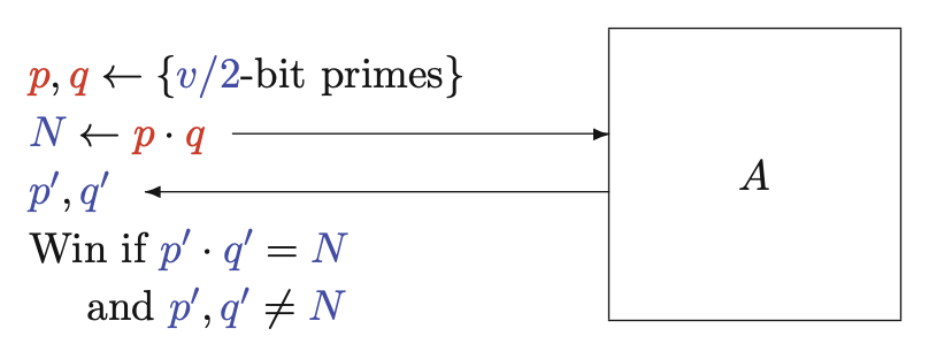
\includegraphics[scale=0.5]{img/game-factor.png}
    \caption{Security game to define the FACTOR problem}
\end{figure}

\subsubsection{Measuring the Adversary's Advantage}

The advantage of the adversary \(A\) in this game is defined as:
\[
\text{Adv}_v^X(A, t) = \Pr\big[A \text{ wins the game } X \text{ for } v = \log_2 N \text{ in time less than } t\big].
\]
Here:
\begin{itemize}
    \item \(v\) is the bit-length of \(N\), representing the problem's complexity.
    \item \(t\) is the allowed time for \(A\).
    \item \(\Pr\) is the probability that \(A\) successfully factors \(N\) under these conditions.
\end{itemize}

\[
\text{Adv}_v^X(A) = 2 \cdot \left| \Pr\big[ A \text{ wins } X \text{ for } v = \log_2 N \big] - \frac{1}{2} \right|
\]
A always wins: 1. A always guesses: 0.

\subsection{Pseudo-Random Functions}
\begin{defn}
A pseudorandom function $F_k(x)$ is a deterministic function that takes an input $x$ and produces an output that is computationally indistinguishable from a truly random function, given only oracle access to the function. No efficient adversary can distinguish between $F_k(x)$ and a truly random function, without knowing the secret key $k$. 
\end{defn}

\textbf{Example in Security Game:}
The game below does not follow Kerkhoff's principle. The adversary always wins, because everything is known. There is no key/security parameter. The adversary can easily check if $F(x) = y$.
\begin{figure}[h!]
    \centering
    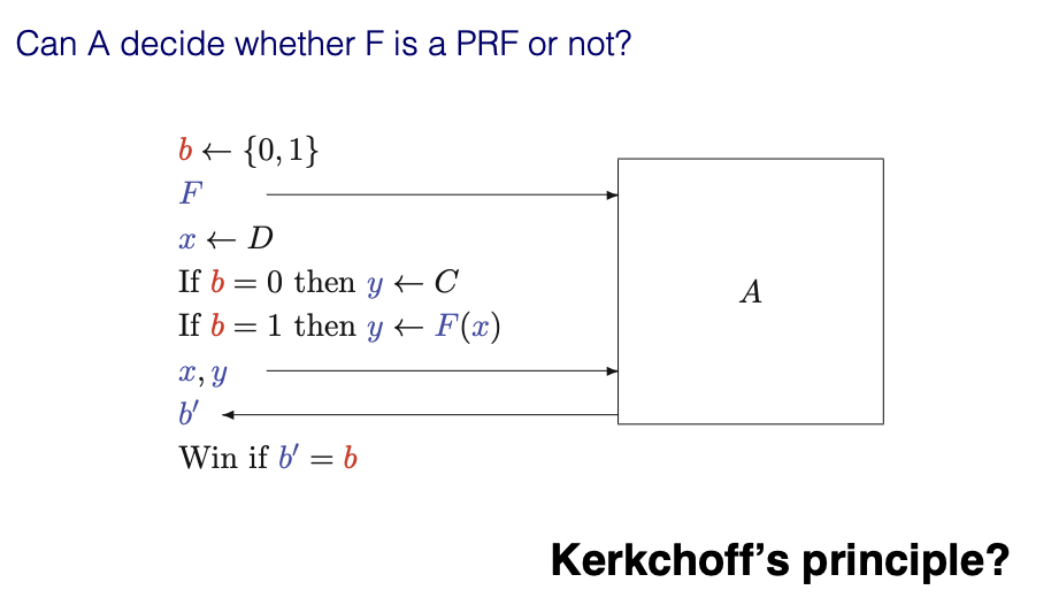
\includegraphics[scale=0.5]{img/PRFbad.png}
    \caption{Security game to define the PRF problem. Here, the adversary always wins!}
\end{figure}

Changing the SG to include a key parameter $k$: we are not having one function $F$, but several functions chosen based on a secret key: $F_k(x)$. The adversary does not know the key. The adversary now has access to an oracle: 

\begin{defn}
An \textbf{oracle} is an abstract, theoretical concept representing a "black box" that provides answers to specific queries according to a defined rule or function. The term is often used to model adversaries' access to resources or information in a controlled manner during security analyses.
\begin{itemize}
    \item The oracle operates according to predefined rules or a specific function (e.g., encryption, decryption, signature generation, or random sampling).
    \item The adversary can query the oracle to obtain information or perform operations, but cannot directly access the oracle's internal workings.
    \item For example, an encryption oracle takes a plaintext as input and outputs the corresponding ciphertext, while a decryption oracle does the reverse.
\end{itemize}
\end{defn}

\begin{figure}[h!]
    \centering
    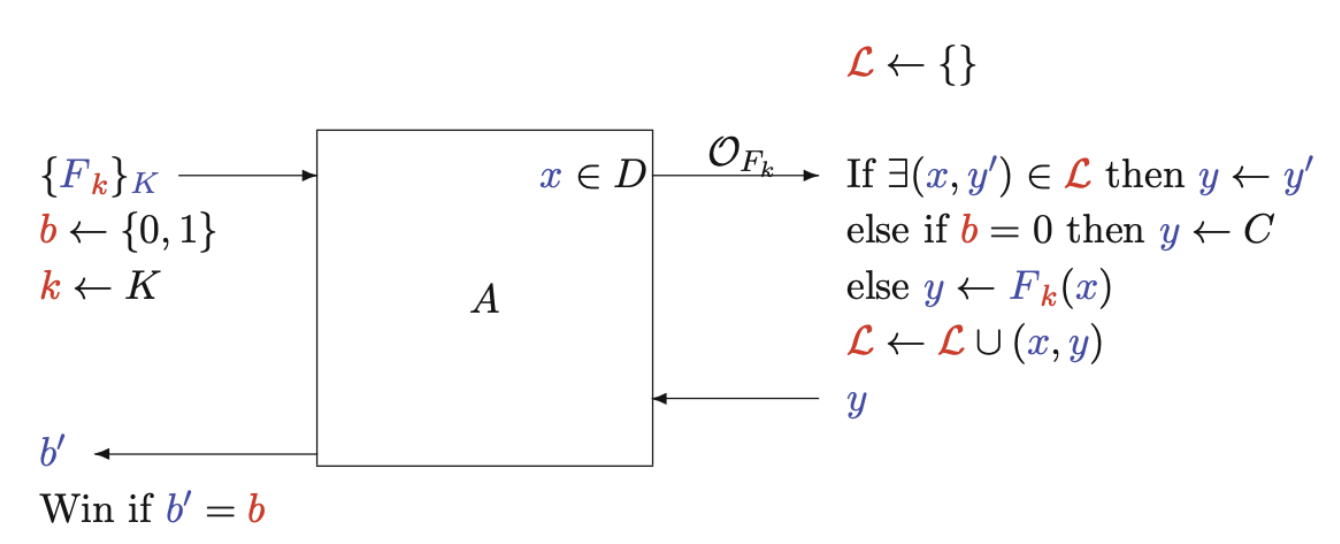
\includegraphics[scale=0.5]{img/PRFfinal.png}
    \caption{The final security game for a PRF}
    \label{PRFfinal}
\end{figure}

\newpage
\textbf{Example: Oracle in a Security Game}
For a PRF function security game, the oracle $\mathcal{O}_k(x)$ behaves as follows:
\begin{itemize}
    \item With secret key $k$, the oracle implements $\mathcal{O}_{F_k}$, where $F_k$ is a pseudorandom function.
    \item Alternatively, the oracle can implement $\mathcal{O}_R$, where $R$ is a truly random function.
    \item The oracle should not give two different answers for the same input $x$. Hence, it has a memory $\mathcal{L}$.
\end{itemize}

The adversary queries the oracle with different $x$ values and observes the outputs. The adversary's goal is to distinguish whether the oracle is implementing a PRF or truly random function, without knowing the secret key $k$. In figure \ref{PRFfinal}, this is indicated by the bit $b$. The adversary wins if they can correctly guess $b$.

\subsubsection{Adversary's Advantage}

The adversary's \textit{advantage} measures how well it can distinguish the oracle's behavior from random guessing. This is formally defined as:

\[
\text{Adv}_{\{F_k\}_K}^{\text{PRF}}(A) = 2 \cdot \left| \Pr\big[A^{O_{F_k}} \text{ wins}\big] - \frac{1}{2} \right|
\]

Key Components:
\begin{itemize}
    \item \( \Pr\big[A^{O_{F_k}} \text{ wins}\big] \): The probability that \( A \) correctly guesses the bit \( b \).
    \item \( \frac{1}{2} \): The probability of guessing \( b \) purely at random.
\end{itemize}

Interpretation:
\begin{itemize}
    \item If \( A \) cannot distinguish \( F_k(x) \) from a random function, its success probability is \( \frac{1}{2} \), meaning \( \text{Adv}_{\{F_k\}_K}^{\text{PRF}}(A) = 0 \).
    \item If \( A \) has some advantage in distinguishing \( F_k(x) \) from random, the value \( \text{Adv} \) increases, indicating the weakness of the PRF.
\end{itemize}

\subsubsection{Why is this important?}
This security game is critical for evaluating whether a function $F_k(x)$ behaves indistinguishably from a truly random function. In cryptographic systems:
\begin{itemize}
    \item Strong PRFs ensure adversaries can't predict outputs or distinguish the function, which is vital for the security of encryption, key derivation, and other cryptographic primitives.
    \item A PRF that is distinguishable from random may leak information or fail to provide the desired security guarantees.
\end{itemize}

\newpage

\subsection{Trapdoor Functions}

\begin{defn}
    A \textbf{one-way function} is a function that is easy to compute in one direction but \emph{hard to invert}.

\begin{itemize}
    \item \textbf{Easy to compute:} Given an input \( x \), it is computationally efficient to calculate \( f(x) \).
    \item \textbf{Hard to invert:} Given \( f(x) \), it is computationally infeasible to find \( x \) (or any \( x' \) such that \( f(x') = f(x) \)) without additional information.
\end{itemize}
\end{defn}

\begin{defn}
    A \textbf{trapdoor} function is a one-way function that is easy to compute in one direction but hard to invert unless a secret "trapdoor" is known. An extra piece of information helps to invert the function, e.g. RSA.
\end{defn}

\begin{figure}[h!]
    \centering
    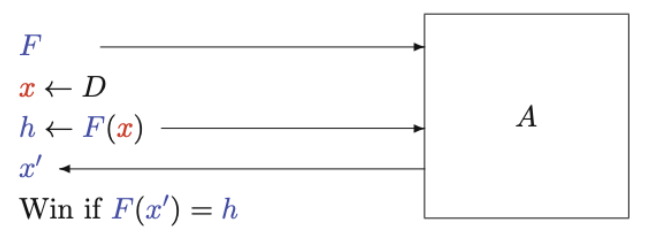
\includegraphics[scale=0.5]{img/OWgame.png}
    \caption{Security game for a one-way function}
    \label{trapdoor}
\end{figure}

\subsection{Public Key Cryptography}
\begin{itemize}
    \item \textbf{Key distribution problem} in symmetric (private key) systems.
    \item A \textbf{key pair} is needed:
    \begin{itemize}
        \item \textbf{Private key} for decryption (only the owner can decrypt).
        \item \textbf{Public key} for encryption (everyone can encrypt).
    \end{itemize}
    \item Public and private keys are linked in a mathematical way:
    \begin{itemize}
        \item Obtaining the private key from the public key is \textbf{NOT easy}.
        \item Obtaining the public key from the private key is \textbf{easy}.
    \end{itemize}
\end{itemize}

The security of an encryption scheme (both symmetric and asymmetric) is dependent on:
\begin{itemize}
    \item The goal of the adversary
    \item The types of attacks allowed
    \item The computational model
\end{itemize}

\subsection{Basic Notions of Security}
Notation and valid encryption: 
\[ \forall k \in \mathbb{K}, \forall m \in \mathbb{P}, d_k(e_k(m)) = m \]
What does it mean for a symmetric encryption scheme to be secure? Adversary should not learn the underlying (plaintext) message.

\subsubsection{OW-PASS attack}
One-wayness under passive attack.
\begin{itemize}
    \item Adversary's Capability: The adversary only observes the encryption of a plaintext message but cannot interact with the encryption mechanism in any way.
    \item Goal: The adversary is given the ciphertext \( c = \text{Enc}(m) \) and attempts to recover the plaintext \( m \).
    \item Assumptions:
    \begin{itemize}
        \item The adversary has no control over the plaintexts being encrypted.
        \item Security is evaluated against passive observers who can only eavesdrop.
    \end{itemize}
    \item Use Case: Suitable for scenarios where the attacker does not have active access to the encryption process.
\end{itemize}

\begin{figure}[h!]
    \centering
    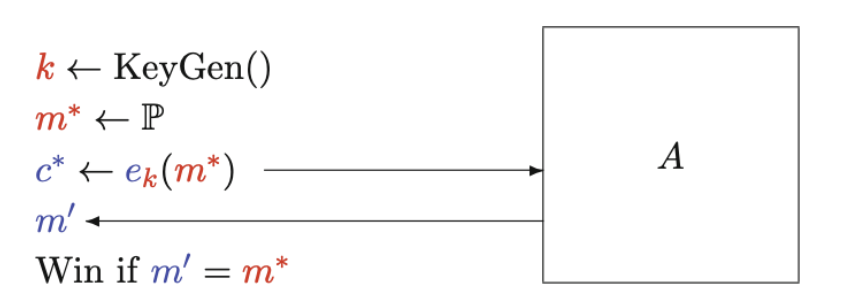
\includegraphics[scale=0.5]{img/OWpass.png}
    \caption{Security game for symmetric key OW-PASS}
\end{figure}


\subsubsection{OW-CPA attack}
OW-PASS is very limiting for the adversary. She should have an encryption oracle. One-Wayness under Chosen Plaintext Attack:
\begin{itemize}
    \item Adversary's Capability: The adversary can interact with the encryption mechanism by choosing plaintexts and obtaining their corresponding ciphertexts.
    \item Goal: The adversary, after observing ciphertexts for chosen plaintexts, attempts to recover the plaintext of a given ciphertext.
    \item Assumptions:
    \begin{itemize}
        \item The adversary can actively query the encryption oracle with plaintexts of their choice.
        \item This security definition is stronger than OW-PA because it assumes a more powerful adversary.
    \end{itemize}
    \item Use Case: Applies to scenarios where the attacker has partial or controlled access to the encryption process, such as in chosen plaintext attacks on public-key cryptography.
\end{itemize}

\begin{figure}[h!]
    \centering
    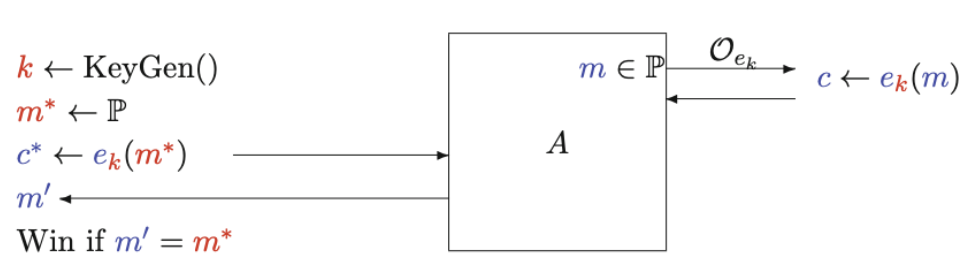
\includegraphics[scale=0.5]{img/OWCPA.png}
    \caption{Security game for symmetric key OW-CPA}
\end{figure}

\subsubsection{OW-CCA attack}
The adversary should be able to decrypt as too (limited number). Thus, One-wayness under Chosen Ciphertext Attack:

\begin{itemize}
    \item Adversary's Capability:
    The adversary is allowed to interact with both the encryption and decryption oracles. Specifically, they can:
    \begin{itemize}
        \item Query the decryption oracle for the decryption of any ciphertext \( c \), except for the target ciphertext \( c^* \).
        \item Query the encryption oracle to obtain the ciphertext for any plaintext \( m \) of their choice.
    \end{itemize}
    
    \item Goal:
    The adversary attempts to recover the plaintext \( m^* \) from a given target ciphertext \( c^* = \text{Enc}(m^*) \).

    \item Assumptions:
    \begin{itemize}
        \item The adversary has powerful capabilities to both query encryption for chosen plaintexts and query decryption for chosen ciphertexts.
        \item The decryption oracle cannot be used directly on the target ciphertext \( c^* \) to prevent trivial success.
    \end{itemize}

    \item Use Case:
    \begin{itemize}
        \item OW-CCA security is crucial for applications requiring strong guarantees against active attackers who can manipulate ciphertexts.
        \item It is relevant in scenarios such as securing communications where adversaries can intercept, modify, and replay ciphertexts.
    \end{itemize}

    \item Key Features:
    \begin{itemize}
        \item Adversary's Advantage: OW-CCA tests the robustness of a cryptographic scheme against the most powerful adversaries who can both observe and manipulate encrypted communications.
        \item Stronger Security: OW-CCA provides stronger guarantees compared to OW-PA and OW-CPA as it accounts for adversaries who have decryption capabilities.
    \end{itemize}
\end{itemize}

\begin{figure}[h!]
    \centering
    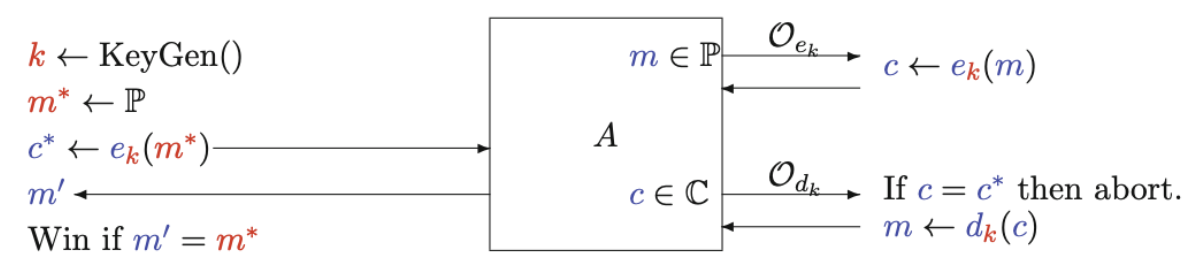
\includegraphics[scale=0.5]{img/OWcca.png}
    \caption{Security game for symmetric key OW-CCA}
\end{figure}

\subsection{Modern Notions of Security}
Before, the attacks assumed that you obtain the whole key. In real life, the adversary can also partially break the system (one bit of the key). The adversary should not be allowed to obtain \textbf{any} information about the plaintext! \\

Perfect secrecy is not practical, because every plaintext needs to have the same probability. To do so, the key needs to be as long as the message.

\begin{defn}
Semantic security: like perfect security but the adversary has polynomially bounded computing power. The adversary cannot extract partial knowledge. 

\[g: M \rightarrow \{0,1\}\] 
\[Pr[g(m) = 1] = Pr[g(m) = 0] = \frac{1}{2}\]
\[ Adv_{\prod}^{\text{SEM}} (S) = 2 \cdot \left| Pr[S(c) = g(d_k(c))] - \frac{1}{2} \right| \]\end{defn}

Semantic security ensures that an adversary cannot learn any meaningful information about a plaintext from its ciphertext, even if they have some prior knowledge about the plaintext. Formally, a cryptosystem is semantically secure if, given a ciphertext, the adversary cannot distinguish between the encryptions of two chosen plaintexts. \\

Semantic security is \emph{difficult to show}! Polynomial security (IND) is easier to show. If a system is IND secure, it is also semantically secure.

\begin{defn}
IND Security: an encryption scheme is \emph{IND-secure} if the ciphertexts of two plaintexts are indistinguishable to an adversary, ensuring that the adversary gains no advantage from observing ciphertexts, even with access to oracles (depending on the attack model).
\end{defn}

IND Security ensures that an adversary cannot distinguish between the ciphertexts of two chosen plaintexts, even if they select the plaintexts themselves. This is a fundamental property of secure encryption. IND Security requires the use of \emph{probabilistic} encryption for public-key encryption schemes to ensure that ciphertexts for the same plaintext look different every time they are encrypted. This randomness prevents adversaries from exploiting patterns in ciphertexts to distinguish between plaintexts.

\subsubsection{IND Security Games} 
The IND framework is defined under different adversarial capabilities: \\

\textbf{IND-CPA} (Indistinguishability under Chosen Plaintext Attack):
\begin{itemize}
    \item The adversary can choose two plaintexts $m_0$ and $m_1$.
    \item A random bit $b$ is chosen, and the ciphertext of $m_b$ is given to the adversary.
    \item The adversary must guess $b$.
    \item Success probability $> \frac{1}{2}$ implies a weakness in the scheme.
\end{itemize}

\textbf{IND-CCA} Indistinguishability under Chosen Ciphertext Attack):
\begin{itemize}
    \item Similar to IND-CPA, but the adversary is also allowed to query a decryption oracle.
    \item The adversary cannot query the decryption oracle for the target ciphertext.
    \item This provides a stronger security guarantee than IND-CPA.
\end{itemize}

\begin{figure}[h!]
    \centering
    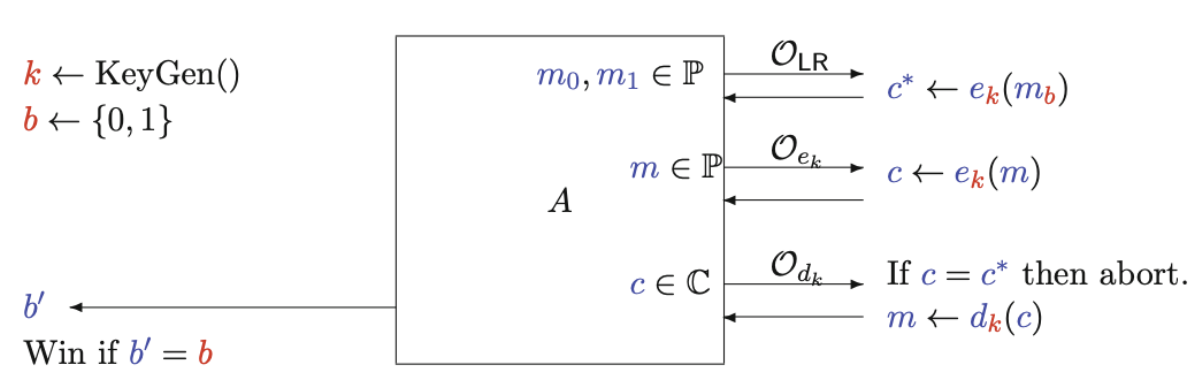
\includegraphics[scale=0.5]{img/INDcca.png}
    \caption{Security game for symmetric key IND-CCA}
    \label{INDcca}
\end{figure}

If the cryptosystem is deterministic, you can fool the oracles. In figure \ref{INDcca}, $\mathcal{O}_{LR}$ will only encrypt one of $m_1, m_2$. You use the other message in the second step $\mathcal{O}_{e_k}$, and check if you receive the same ciphertext as in step 1.
The decryption oracle $\mathcal{O}_{d_k}$ can be fooled if there is a relationship between the plain text and the cypertext. This is possible in homomorphic encryption.
For secure communication, homomorphism is not appreciated. But we have it because in public cryptosystems we rely on mathematically difficult problems.
\begin{defn}
An encryption algorithm is secure if it is semantically secure against a CPA attack.
\end{defn}

\begin{defn}
An encryption algorithm is secure if it is IND-CCA secure.
\end{defn}

\begin{thm}
A system which is IND-PASS secure must be semanticallt secure against passive adversaries.

\[ \prod \text{ is IND-CCA} \Rightarrow \prod \text{ is IND-CPA} \Rightarrow \prod \text{ is IND-PASS} \] 
\[ \prod \text{ is IND-XXX} \Rightarrow \prod \text{ is OW-XXX} \]
\end{thm}

\subsection{Other Notions of Security}
\Comment{Add definitions here from slides}

\subsection{Random Oracle Model}
\Comment{Finish later}